\chapter{WebAIM: Screen Reader User Survey \#10 Results}\label{chap:webaim-survey}

\section{Introduction}\label{sec:intro}

In December 2023 and January 2024, WebAIM surveyed preferences of screen reader users. We received 1539 valid responses. This was a follow-up to 9 previous surveys conducted between January 2009 and June 2021.

A few disclaimers and notices:
\begin{itemize}
    \item Totals may not equal 100\% due to rounding.
    \item Total responses (n) for each question may not equal 1539 due to some respondents not answering a particular question.
    \item The sample was not controlled and may not represent all screen reader users.
    \item We hope to conduct additional surveys of this nature again in the future. If you have recommendations or questions that you would like us to ask, please contact us.
\end{itemize}

Supported by BrowserStack. Support for this research is funded in part by a donation from BrowserStack.

\section{Demographics}\label{sec:demographics}

\subsection{Region}\label{subsec:region}
The following table shows the distribution of respondents by region.

\begin{longtblr}[
  caption = {Survey Respondents by Region},
  label = {tab:region},
  note = {This table provides an accessible summary of the geographic distribution of survey respondents. It is designed to help readers understand the global reach and diversity of the survey audience, with emphasis on representation outside North America. The table supports interpretation of regional differences in screen reader usage and is structured for clarity and ease of navigation for all users, including those using assistive technology.},
]{
  colspec = {Q[l,m] Q[l,m] Q[l,m]},
  rowhead = 1
}
\hline
Region & \# of respondents & \% of respondents \\
\hline
North America & 717 & 47.2\% \\
Europe & 467 & 30.7\% \\
Asia & 97 & 6.4\% \\
South America & 96 & 6.3\% \\
Africa/Middle East & 73 & 4.8\% \\
Australia and Oceania & 50 & 3.3\% \\
Central America and Caribbean & 20 & 1.3\% \\
\hline
\end{longtblr}
\par

This survey saw a majority of respondents from outside North America, thus providing better representation of the global screen reader user audience. When survey responses were notably different between regions, this is noted below.

\subsection{Age}\label{subsec:age}
The following table shows the age distribution of respondents.

\begin{longtblr}[
  caption = {Survey Respondents by Age},
  label = {tab:age},
  note = {This table offers an accessible overview of the age distribution among survey respondents. It is intended to help readers interpret generational trends in screen reader usage and technology adoption. The table is structured for clarity and is accompanied by descriptive context to support users of all abilities, including those using screen readers.},
]{
  colspec = {Q[l,m] Q[l,m] Q[l,m]},
  rowhead = 1
}
\hline
Age & \# of respondents & \% of respondents \\
\hline
Below 20 & 94 & 6.1\% \\
21--40 & 584 & 37.9\% \\
41--60 & 553 & 35.9\% \\
60+ & 308 & 20.0\% \\
\hline
\end{longtblr}
\par

\subsection{Disability}\label{subsec:disability}
The following table shows whether respondents use a screen reader due to a disability.

\begin{longtblr}[
  caption = {Screen Reader Use Due to Disability},
  label = {tab:disability},
  note = {This table provides accessible information on whether respondents use a screen reader due to a disability. It is designed to help readers understand the proportion of users with and without disabilities and to highlight differences in their experiences and responses. The table is formatted for clarity and accessibility, supporting interpretation by all readers, including those using assistive technology.},
]{
  colspec = {Q[l,m] Q[l,m] Q[l,m]},
  rowhead = 1
}
\hline
Response & \# of respondents & \% of respondents \\
\hline
Yes & 1372 & 89.9\% \\
No & 154 & 10.1\% \\
\hline
\end{longtblr}
\par

Responses are predominantly very similar for respondents with and without disabilities. Any notable differences are indicated below to highlight differences in practices or perceptions between disabled and non-disabled respondents.

\subsection{Disability Types}\label{subsec:disability-types}
The following table shows the types of disabilities reported by respondents.

\begin{longtblr}[
  caption = {Types of Disabilities Reported},
  label = {tab:disability-types},
  note = {This table presents an accessible summary of the types of disabilities reported by survey respondents, including blindness, low vision, cognitive, motor, and hearing impairments. It also notes the prevalence of multiple disabilities. The table is structured to provide clear, descriptive context for all readers, including those using assistive technology, and supports interpretation of the diversity within the respondent population.},
]{
  colspec = {Q[l,m] Q[l,m] Q[l,m]},
  rowhead = 1
}
\hline
Response & \# of respondents & \% of respondents \\
\hline
Blindness & 1179 & 76.6\% \\
Low Vision/Visually-Impaired & 306 & 19.9\% \\
Cognitive or Learning & 80 & 5.2\% \\
Deafness/Hard-of-Hearing & 104 & 6.8\% \\
Motor & 34 & 2.2\% \\
Other & 75 & 4.9\% \\
\hline
\end{longtblr}
\par

257 respondents (16.7\%) reported multiple disabilities. 81 respondents (5.3\%) reported being both deaf/hard-of-hearing and blind.

\subsection{Screen Reader Proficiency}\label{subsec:sr-proficiency}
The following table shows respondents' self-rated screen reader proficiency.

\begin{longtblr}[
  caption = {Screen Reader Proficiency},
  label = {tab:sr-proficiency},
  note = {This table provides an accessible summary of respondents’ self-assessed proficiency with screen readers, distinguishing between advanced, intermediate, and beginner users. It highlights differences based on disability status and is formatted for clarity and ease of interpretation for all readers, including those using assistive technology.},
]{
  colspec = {Q[l,m] Q[l,m] Q[l,m]},
  rowhead = 1
}
\hline
Response & \# of respondents & \% of respondents \\
\hline
Advanced & 888 & 58.3\% \\
Intermediate & 548 & 36.0\% \\
Beginner & 87 & 5.7\% \\
\hline
\end{longtblr}
\par

Those who use screen readers due to a disability reported themselves as more proficient with screen readers—63\% of those with disabilities considered their proficiency to be ``Advanced'' compared to only 18.2\% of those without disabilities.

\subsection{Internet Proficiency}
The following table shows respondents' self-rated Internet proficiency.

\begin{longtblr}[
  caption = {Internet Proficiency},
  label = {tab:internet-proficiency},
  note = {This table offers an accessible overview of respondents’ self-rated proficiency using the Internet, providing insight into their comfort and skill level with online technologies. It highlights differences between disabled and non-disabled users and is structured for clarity and accessibility for all readers, including those using assistive technology.},
]{
  colspec = {Q[l,m] Q[l,m] Q[l,m]},
  rowhead = 1
}
\hline
Response & \# of respondents & \% of respondents \\
\hline
Advanced & 1091 & 71.8\% \\
Intermediate & 401 & 26.4\% \\
Beginner & 28 & 1.8\% \\
\hline
\end{longtblr}
\par

Those without disabilities rated themselves as more proficient than those with disabilities.

\section{Primary Desktop/Laptop Screen Reader}

The following table shows the primary desktop/laptop screen reader used by respondents.

\begin{longtblr}[
  caption = {Primary Desktop/Laptop Screen Reader},
  label = {tab:primary-sr},
  note = {This table provides an accessible summary of the primary desktop or laptop screen reader used by respondents. It highlights trends in popularity among major screen readers and notes regional and disability-related usage patterns. The table is formatted for clarity and ease of navigation for all users, including those using assistive technology.},
]{
  colspec = {Q[l,m] Q[l,m] Q[l,m]},
  rowhead = 1
}
\hline
Response & \# of respondents & \% of respondents \\
\hline
JAWS & 619 & 40.5\% \\
NVDA & 577 & 37.7\% \\
VoiceOver & 148 & 9.7\% \\
Dolphin SuperNova & 57 & 3.7\% \\
ZoomText/Fusion & 41 & 2.7\% \\
Orca & 36 & 2.4\% \\
Narrator & 10 & 0.7\% \\
Other & 41 & 2.7\% \\
\hline
\end{longtblr}
\par

\begin{figure}[htbp]
\centering
\tagstructbegin{tag=Figure}
%\imgalt{This line chart presents the percentage of survey respondents identifying each screen reader as their primary choice from 2009 to 2024. JAWS and NVDA show alternating dominance, with JAWS leading early and NVDA increasing steadily. VoiceOver maintains a smaller but consistent share. The chart highlights shifts in user preference and the emergence of new screen readers over time.}
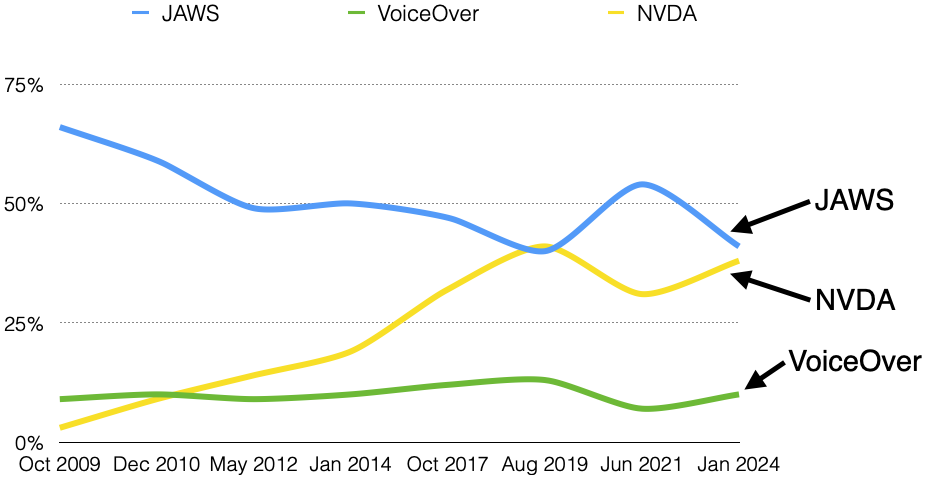
\includegraphics[alt={This line chart presents the percentage of survey respondents identifying each screen reader as their primary choice from 2009 to 2024. JAWS and NVDA show alternating dominance, with JAWS leading early and NVDA increasing steadily. VoiceOver maintains a smaller but consistent share. The chart highlights shifts in user preference and the emergence of new screen readers over time.}]{images/SR-1.png}
\caption{Historical trends for primary screen reader usage since October 2009.}
\label{fig:sr1}
\tagstructend
\end{figure}

Historically JAWS usage had been in decline until 2019 when JAWS and NVDA were nearly the same. The 2021 survey saw an increase in JAWS usage and decrease in NVDA usage, but in 2024 the usage of both are again nearly the same at 41\% for JAWS and 38\% for NVDA.

Respondents with disabilities are more likely to use JAWS and NVDA and less likely to use VoiceOver as their primary screen reader than respondents without disabilities. 8.2\% of respondents with disabilities primarily use VoiceOver (up from 5.5\% in 2021), compared to 23.7\% of respondents without disabilities.

Primary usage varied greatly by region. JAWS usage was higher than NVDA in North America (55.5\% vs. 24.0\%) and Australia (45.8\% vs. 37.5\%), though JAWS usage was lower than NVDA in Europe (29.7\% vs. 37.2\%), Africa/Middle East (23.3\% vs. 69.9\%), and Asia (22.9\% vs. 70.8\%).

Beyond the three most popular primary screen readers, other screen readers comprised a total of 12.2\% of usage.

\section{Screen Readers Commonly Used}

The following table shows desktop/laptop screen readers commonly used by respondents.

\begin{longtblr}[
  caption = {Screen Readers Commonly Used},
  label = {tab:sr-commonly-used},
  note = {This table presents an accessible overview of all desktop/laptop screen readers commonly used by respondents, illustrating the prevalence of multi-screen reader usage and changes in adoption over time. The table is structured for clarity and supports interpretation by all readers, including those using assistive technology.},
]{
  colspec = {Q[l,m] Q[l,m] Q[l,m]},
  rowhead = 1
}
\hline
Response & \# of respondents & \% of respondents \\
\hline
NVDA & 1009 & 65.6\% \\
JAWS & 931 & 60.5\% \\
VoiceOver & 675 & 43.9\% \\
Narrator & 574 & 37.3\% \\
Orca & 127 & 8.3\% \\
ZoomText/Fusion & 115 & 7.5\% \\
Dolphin SuperNova & 83 & 5.4\% \\
ChromeVox & 59 & 3.8\% \\
System Access or System Access to Go & 28 & 1.8\% \\
Window-Eyes & 18 & 1.2\% \\
Other & 79 & 5.1\% \\
\hline
\end{longtblr}
\par

\begin{figure}[htbp]
\centering
\tagstructbegin{tag=Figure}
%\imgalt{This bar chart compares the percentage of respondents reporting use of various screen readers (JAWS, NVDA, VoiceOver, and others) across several survey years. JAWS and NVDA are the most commonly used, with NVDA showing significant growth. VoiceOver usage remains steady, while other screen readers have lower and declining usage rates.}
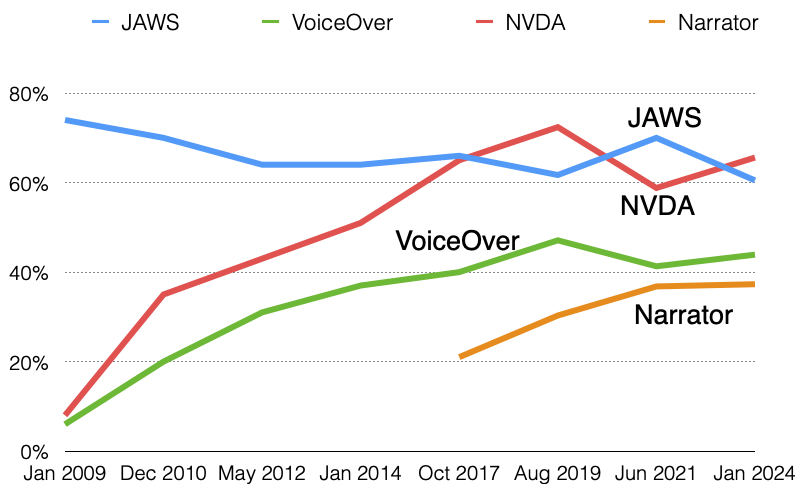
\includegraphics[alt={This bar chart compares the percentage of respondents reporting use of various screen readers (JAWS, NVDA, VoiceOver, and others) across several survey years. JAWS and NVDA are the most commonly used, with NVDA showing significant growth. VoiceOver usage remains steady, while other screen readers have lower and declining usage rates.}]{images/SR-2.png}
\caption{Chart of screen reader usage over time.}
\label{fig:sr2}
\tagstructend
\end{figure}

NVDA is again the most commonly used screen reader at 65.6\% of respondents outpacing JAWS at 60.5\%. Narrator—freely available in Windows for several years—is the primary screen reader of only 0.7\% of respondents, but is commonly used by 37.3\% of respondents.

71.6\% of respondents use more than one desktop/laptop screen reader. 43\% use three or more, and 17.4\% use four or more different screen readers. VoiceOver users most commonly use additional screen readers.

\section{Browsers}

The following table shows the browser most often used with the primary screen reader.

\begin{longtblr}[
  caption = {Primary Browser Used with Screen Reader},
  label = {tab:browser},
  note = {This table provides an accessible summary of the web browsers most frequently used with respondents’ primary screen readers. It tracks browser trends and preferences among users and is formatted for clarity and ease of interpretation for all readers, including those using assistive technology.},
]{
  colspec = {Q[l,m] Q[l,m] Q[l,m]},
  rowhead = 1
}
\hline
Response & \# of respondents & \% of respondents \\
\hline
Chrome & 795 & 52.3\% \\
Microsoft Edge & 294 & 19.3\% \\
Firefox & 243 & 16.0\% \\
Safari & 121 & 8.0\% \\
Internet Explorer & 14 & 0.9\% \\
Other & 54 & 3.6\% \\
\hline
\end{longtblr}
\par

\begin{figure}[htbp]
\centering
\tagstructbegin{tag=Figure}
%\imgalt{This line chart illustrates the changing preferences for web browsers among screen reader users from 2009 to 2024. Chrome shows a marked increase in usage, overtaking Internet Explorer and Firefox. Edge usage rises in recent years, while Internet Explorer declines sharply. The chart emphasizes the shift toward modern browsers and the impact on accessibility.}
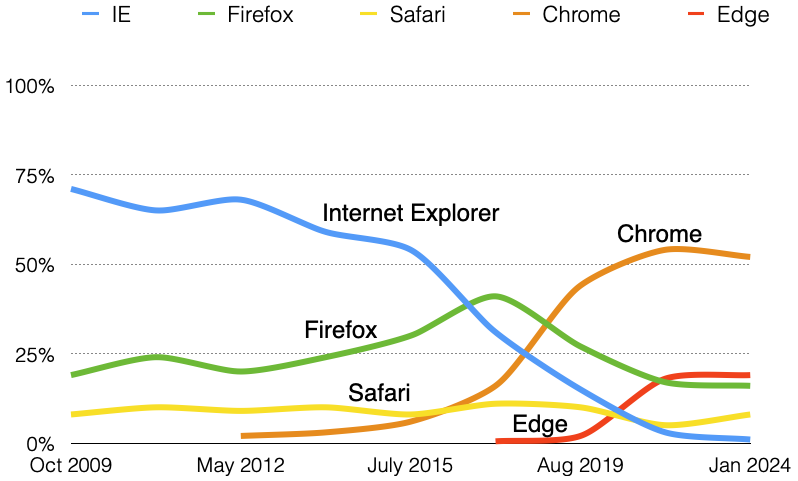
\includegraphics[alt={This line chart illustrates the changing preferences for web browsers among screen reader users from 2009 to 2024. Chrome shows a marked increase in usage, overtaking Internet Explorer and Firefox. Edge usage rises in recent years, while Internet Explorer declines sharply. The chart emphasizes the shift toward modern browsers and the impact on accessibility.}]{images/browsers.png}
\caption{Historical trends for primary browser usage.}
\label{fig:browsers}
\tagstructend
\end{figure}

Browser usage remains mostly unchanged since 2021, with Chrome and Internet Explorer seeing small decreases in usage and Safari a small increase in usage.

\section{Screen Reader / Browser Combinations}

The following table shows the most common screen reader and browser combinations.

\begin{longtblr}[
  caption = {Most Common Screen Reader and Browser Combinations},
  label = {tab:sr-browser-combo},
  note = {This table presents an accessible overview of the most popular combinations of screen readers and browsers among respondents. It highlights the diversity of technology setups and the most frequently paired solutions. The table is structured for clarity and supports interpretation by all readers, including those using assistive technology.},
]{
  colspec = {Q[l,m] Q[l,m] Q[l,m]},
  rowhead = 1
}
\hline
Screen Reader \& Browser & \# of respondents & \% of respondents \\
\hline
JAWS with Chrome & 373 & 24.7\% \\
NVDA with Chrome & 323 & 21.3\% \\
JAWS with Edge & 173 & 11.4\% \\
NVDA with Firefox & 152 & 10.0\% \\
VoiceOver with Safari & 107 & 7.0\% \\
NVDA with Edge & 75 & 5.0\% \\
JAWS with Firefox & 39 & 2.6\% \\
VoiceOver with Chrome & 30 & 2.0\% \\
Orca with Firefox & 29 & 1.9\% \\
Dolphin SuperNova with Chrome & 24 & 1.6\% \\
ZoomText/Fusion with Chrome & 18 & 1.2\% \\
ZoomText/Fusion with Edge & 16 & 1.1\% \\
Other combinations & 154 & 10.2\% \\
\hline
\end{longtblr}
\par

There are \textbf{many} combinations of browsers and screen readers in use, with JAWS with Chrome the most common.

\section{Operating System}

The following table shows the operating system used with the primary desktop/laptop screen reader.

\begin{longtblr}[
  caption = {Operating System Used with Primary Screen Reader},
  label = {tab:os},
  note = {This table presents the operating systems used with respondents’ primary screen readers, showing the dominance of Windows and noting differences in OS preference by disability status.},
]{
  colspec = {Q[l,m] Q[l,m] Q[l,m]},
  rowhead = 1
}
\hline
Response & \# of respondents & \% of respondents \\
\hline
Windows & 1311 & 86.1\% \\
Mac & 146 & 9.6\% \\
Linux & 44 & 2.9\% \\
Other & 21 & 1.4\% \\
\hline
\end{longtblr}
\par

Respondents without disabilities were nearly 3 times more likely to use Mac OS than respondents with disabilities.

\section{JavaScript}

The following table shows whether JavaScript was enabled.

\begin{longtblr}[
  caption = {JavaScript Enabled},
  label = {tab:js-enabled},
  note = {This table indicates whether respondents had JavaScript enabled during the survey, reflecting the near-universal support for JavaScript among screen reader users.},
]{
  colspec = {Q[l,m] Q[l,m]},
  rowhead = 1
}
\hline
Response & \% of respondents \\
\hline
Yes & 99.8\% \\
No & 0.2\% \\
\hline
\end{longtblr}
\par

JavaScript support was detected with the survey form submission. Nearly all respondents had JavaScript enabled.

\section{Reason for Use}

The following table shows the main reason for using the primary screen reader.

\begin{longtblr}[
  caption = {Main Reason for Using Primary Screen Reader},
  label = {tab:reason-use},
  note = {This table explores the main reasons respondents use their chosen primary screen reader, including comfort, features, availability, cost, and support, and notes shifts in these motivations over time.},
]{
  colspec = {Q[l,m] Q[l,m] Q[l,m]},
  rowhead = 1
}
\hline
Response & \# of respondents & \% of respondents \\
\hline
Existing Comfort/Expertise & 685 & 45.8\% \\
Features & 396 & 26.5\% \\
Availability & 175 & 11.7\% \\
Cost & 137 & 9.2\% \\
Support & 104 & 6.9\% \\
\hline
\end{longtblr}
\par

Existing comfort and features went down slightly, and Availability, Cost, and Support went up slightly.

\section{Screen Reader Satisfaction}

The following table shows satisfaction with the primary screen reader.

\begin{longtblr}[
  caption = {Screen Reader Satisfaction},
  label = {tab:sr-satisfaction},
  note = {This table summarizes satisfaction levels with respondents’ primary screen readers, breaking down responses by screen reader brand and highlighting overall satisfaction trends.},
]{
  colspec = {Q[l,m] Q[l,m] Q[l,m]},
  rowhead = 1
}
\hline
Response & \# of respondents & \% of respondents \\
\hline
Very satisfied & 966 & 63.8\% \\
Somewhat satisfied & 475 & 31.4\% \\
Slightly satisfied & 56 & 3.7\% \\
Not satisfied & 18 & 1.2\% \\
\hline
\end{longtblr}
\par

Respondents indicating that they are very or somewhat satisfied by their primary screen reader:
\begin{itemize}
    \item NVDA - 97.6\%
    \item JAWS - 95.6\%
    \item VoiceOver - 92.4\%
    \item Narrator - 88.9\%
\end{itemize}

\section{Home vs. Work}

The following table shows whether respondents use a different screen reader at work or school than at home.

\begin{longtblr}[
  caption = {Different Screen Reader at Work/School vs. Home},
  label = {tab:home-vs-work},
  note = {This table shows whether respondents use different screen readers at work/school compared to home, providing insight into context-dependent technology choices and notable differences among screen reader brands.},
]{
  colspec = {Q[l,m] Q[l,m] Q[l,m]},
  rowhead = 1
}
\hline
Response & \# of respondents & \% of respondents \\
\hline
Yes & 266 & 18.6\% \\
No & 1165 & 81.4\% \\
\hline
\end{longtblr}
\par

31\% of VoiceOver users reported using a different screen reader at work/school vs. home, versus 19\% for NVDA, and 15\% for JAWS.

\section{Braille Output}

The following table shows whether respondents use braille output with their screen reader.

\begin{longtblr}[
  caption = {Braille Output Usage},
  label = {tab:braille-output},
  note = {This table reports the proportion of respondents who use braille output with their screen reader, noting trends in braille adoption and differences among screen reader brands.},
]{
  colspec = {Q[l,m] Q[l,m] Q[l,m]},
  rowhead = 1
}
\hline
Response & \# of respondents & \% of respondents \\
\hline
Yes & 510 & 38\% \\
No & 833 & 62\% \\
\hline
\end{longtblr}
\par

Braille usage at 38\% is up slightly from 33.3\% in 2017 and 27.7\% in 2012. 54.2\% of VoiceOver users used Braille compared to 42.4\% of NVDA users and 35.1\% of JAWS users.

\section{Free/Low-cost vs. Commercial}

The following table shows whether respondents see free or low-cost desktop screen readers as viable alternatives to commercial screen readers.

\begin{longtblr}[
  caption = {Perception of Free/Low-cost Screen Readers},
  label = {tab:free-vs-commercial},
  note = {This table assesses respondents’ views on the viability of free or low-cost screen readers compared to commercial options, highlighting differences in perception by screen reader brand and proficiency level.},
]{
  colspec = {Q[l,m] Q[l,m] Q[l,m]},
  rowhead = 1
}
\hline
Response & \# of respondents & \% of respondents \\
\hline
Yes & 1171 & 78.1\% \\
No & 181 & 12.1\% \\
I Don't Know & 148 & 9.9\% \\
\hline
\end{longtblr}
\par

Only 67\% of JAWS users answered ``Yes'' compared to an overwhelming 91\% of VoiceOver users and 94\% of NVDA users. Respondents with ``Advanced'' screen reader proficiency were also more favorable of free/low-cost screen readers.

\section{Mobile Screen Readers}

\subsection{Mobile Usage}

The following table shows whether respondents use a screen reader on a mobile device.

\begin{longtblr}[
  caption = {Mobile Screen Reader Usage},
  label = {tab:mobile-usage},
  note = {This table shows the proportion of respondents who use a screen reader on mobile devices, reflecting the widespread adoption of mobile screen readers among users.},
]{
  colspec = {Q[l,m] Q[l,m] Q[l,m]},
  rowhead = 1
}
\hline
Response & \# of respondents & \% of respondents \\
\hline
Yes & 1379 & 91.3\% \\
No & 132 & 8.7\% \\
\hline
\end{longtblr}
\par

\subsection{Mobile Platforms}

The following table shows the primary mobile/tablet platform used.

\begin{longtblr}[
  caption = {Primary Mobile/Tablet Platform},
  label = {tab:mobile-platform},
  note = {This table lists the primary mobile or tablet platforms used by respondents, showing the dominance of iOS and Android and tracking changes in platform preference over time.},
]{
  colspec = {Q[l,m] Q[l,m] Q[l,m]},
  rowhead = 1
}
\hline
Response & \# of respondents & \% of respondents \\
\hline
Apple iPhone, iPad, or iPod touch & 1048 & 70.6\% \\
Android & 409 & 27.6\% \\
Chrome OS & 7 & 0.5\% \\
Other & 19 & 1.3\% \\
\hline
\end{longtblr}
\par

\begin{figure}[htbp]
\centering
\tagstructbegin{tag=Figure}
%\imgalt{This line chart displays the percentage of screen reader users reporting use of mobile platforms from 2009 to 2024. iOS consistently leads, with Android usage gradually increasing. Other platforms remain low and stable. The chart highlights the dominance of iOS and the growing adoption of Android among users with accessibility needs.}
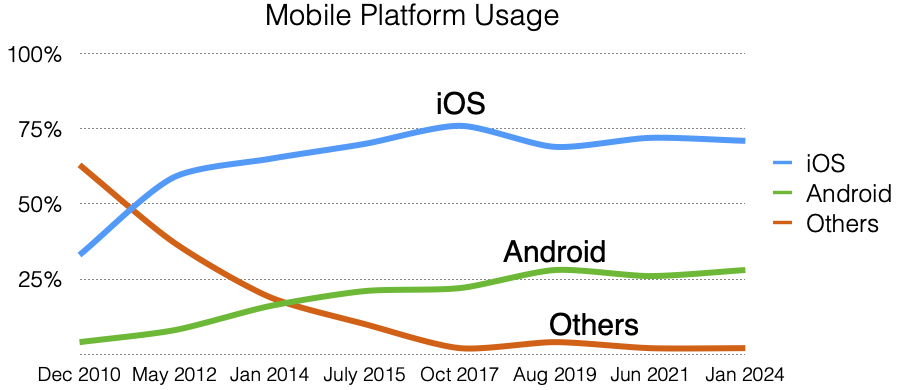
\includegraphics[ alt={This line chart displays the percentage of screen reader users reporting use of mobile platforms from 2009 to 2024. iOS consistently leads, with Android usage gradually increasing. Other platforms remain low and stable. The chart highlights the dominance of iOS and the growing adoption of Android among users with accessibility needs.}]{images/mobile2.png}
\caption{Historical trends for mobile platform usage.}
\label{fig:mobile2}
\tagstructend
\end{figure}

iOS devices continue to dominate the mobile screen reader market. Usage of platforms other than iOS and Android combined represent only 1.8\% of reported usage.

\subsection{Mobile Screen Readers Used}

The following table shows mobile/tablet screen readers commonly used.

\begin{longtblr}[
  caption = {Mobile/Tablet Screen Readers Commonly Used},
  label = {tab:mobile-sr-used},
  note = {This table identifies the mobile and tablet screen readers most commonly used by respondents, highlighting the prevalence of VoiceOver and TalkBack and noting other options in use.},
]{
  colspec = {Q[l,m] Q[l,m]},
  rowhead = 1
}
\hline
Response & \% of respondents \\
\hline
VoiceOver & 70.6\% \\
TalkBack & 34.7\% \\
Commentary/Jieshuo & 10.1\% \\
Voice Assistant & 6.0\% \\
VoiceView & 5.9\% \\
Mobile Accessibility for Android & 4.9\% \\
Mobile Speak & 1.0\% \\
Nuance Talks & 1.0\% \\
IDEAL & 0.5\% \\
Other & 4.7\% \\
\hline
\end{longtblr}
\par

\subsection{Primary Mobile Browser}

The following table shows the primary mobile web browser used.

\begin{longtblr}[
  caption = {Primary Mobile Web Browser},
  label = {tab:mobile-browser},
]{
  colspec = {Q[l,m] Q[l,m] Q[l,m]},
  rowhead = 1
}
\hline
Response & \# of respondents & \% of respondents \\
\hline
Safari & 854 & 58.2\% \\
Chrome & 410 & 27.9\% \\
Firefox & 68 & 4.6\% \\
IE or Edge Mobile & 39 & 2.7\% \\
Android Browser & 23 & 1.6\% \\
Samsung Browser & 16 & 1.1\% \\
Other & 57 & 3.9\% \\
\hline
\end{longtblr}
\par

Safari saw a small decrease in usage while Chrome had a slight increase in usage since 2021.

\subsection{Mobile vs. Desktop/Laptop Usage}

The following table shows whether respondents use a screen reader most often on a desktop/laptop computer or a mobile/tablet device.

\begin{longtblr}[
  caption = {Device Most Often Used for Screen Reader},
  label = {tab:device-most-used},
]{
  colspec = {Q[l,m] Q[l,m] Q[l,m]},
  rowhead = 1
}
\hline
Response & \# of respondents & \% of respondents \\
\hline
Desktop/laptop & 610 & 40.2\% \\
Mobile/tablet and desktop/laptop about the same & 751 & 49.5\% \\
Mobile/tablet device & 155 & 10.2\% \\
\hline
\end{longtblr}
\par

There was almost no change to responses to this question compared to the 2019 survey.

\subsection{Mobile App vs Web Site Usage}

The following table shows whether respondents prefer mobile apps or web sites for common online tasks.

\begin{longtblr}[
  caption = {Preference for Mobile App vs Web Site},
  label = {tab:app-vs-web},
]{
  colspec = {Q[l,m] Q[l,m] Q[l,m]},
  rowhead = 1
}
\hline
Response & \# of respondents & \% of respondents \\
\hline
app & 852 & 58\% \\
web & 618 & 42\% \\
\hline
\end{longtblr}
\par

Respondents indicated that they are much more likely to use a mobile app than a web site for common online tasks. The preference for mobile app usage increased to 58\% in 2024, up from 51.8\% in 2021 and 46\% in 2017.

\section{Web Accessibility Progress}

The following table shows respondents' feelings regarding the accessibility of web content over the previous year.

\begin{longtblr}[
  caption = {Perception of Web Accessibility Progress},
  label = {tab:web-access-progress},
]{
  colspec = {Q[l,m] Q[l,m] Q[l,m]},
  rowhead = 1
}
\hline
Response & \# of respondents & \% of respondents \\
\hline
Web content has become more accessible & 522 & 34.6\% \\
Web content accessibility has not changed & 707 & 46.8\% \\
Web content has become less accessible & 281 & 18.6\% \\
\hline
\end{longtblr}
\par

Perception of the state of web accessibility decreased slightly since 2021. Respondents without disabilities tend to be more positive about recent progress (45.9\% thought it has become more accessible) than those with disabilities (33.4\% thought it has become more accessible).

\section{Impacts on Accessibility}

The following table shows what respondents think would have a bigger impact on improvements to web accessibility.

\begin{longtblr}[
  caption = {Biggest Impact on Web Accessibility},
  label = {tab:impact-accessibility},
]{
  colspec = {Q[l,m] Q[l,m] Q[l,m]},
  rowhead = 1
}
\hline
Response & \# of respondents & \% of respondents \\
\hline
Better assistive technology & 213 & 14.1\% \\
Better (more accessible) web sites & 1298 & 85.9\% \\
\hline
\end{longtblr}
\par

Over time, more respondents have answered ``better web sites'' to this question.

\section{Descriptions in Virtual Meetings}

The following table shows whether respondents think a person should describe what they look like during a virtual meeting or webinar.

\begin{longtblr}[
  caption = {Preference for Descriptions in Virtual Meetings},
  label = {tab:virtual-meeting-desc},
]{
  colspec = {Q[l,m] Q[l,m] Q[l,m]},
  rowhead = 1
}
\hline
Response & \# of respondents & \% of respondents \\
\hline
Yes & 363 & 31.8\% \\
No & 779 & 68.2\% \\
\hline
\end{longtblr}
\par

The majority (68.2\%) of respondents do not prefer descriptions of appearances in online meetings.

\section{Landmarks/Regions}

The following table shows how often respondents navigate by landmarks/regions in their screen reader.

\begin{longtblr}[
  caption = {Frequency of Landmark/Region Navigation},
  label = {tab:landmarks},
]{
  colspec = {Q[l,m] Q[l,m] Q[l,m]},
  rowhead = 1
}
\hline
Response & \# of respondents & \% of respondents \\
\hline
Whenever they're available & 268 & 17.9\% \\
Often & 208 & 13.9\% \\
Sometimes & 471 & 31.5\% \\
Seldom & 309 & 20.6\% \\
Never & 241 & 16.1\% \\
\hline
\end{longtblr}
\par

After steady decreases in the frequent usage of landmarks/regions was seen from 2014 (43.8\%) to 2021 (25.6\%). In 2024 the reported frequent usage has now increased to 31.8\%.

\section{Finding Information}

The following table shows how respondents most often try to find information on a lengthy web page.

\begin{longtblr}[
  caption = {Preferred Method for Finding Information on Lengthy Web Pages},
  label = {tab:finding-info},
]{
  colspec = {Q[l,m] Q[l,m] Q[l,m]},
  rowhead = 1
}
\hline
Response & \# of respondents & \% of respondents \\
\hline
Navigate through the headings on the page & 1082 & 71.6\% \\
Read through the page & 96 & 6.4\% \\
Use the Find feature & 205 & 13.6\% \\
Navigate through the links of the page & 72 & 4.8\% \\
Navigate through the landmarks/regions of the page & 56 & 3.7\% \\
\hline
\end{longtblr}
\par

The usage of headings for finding information has increased over time, and it remains the predominant method.

\section{Heading Levels}

The following table shows how useful heading levels are for navigation.

\begin{longtblr}[
  caption = {Usefulness of Heading Levels for Navigation},
  label = {tab:heading-levels},
]{
  colspec = {Q[l,m] Q[l,m] Q[l,m]},
  rowhead = 1
}
\hline
Response & \# of respondents & \% of respondents \\
\hline
Very useful & 855 & 57.0\% \\
Somewhat useful & 477 & 31.8\% \\
Not very useful & 113 & 7.5\% \\
Not at all useful & 27 & 1.8\% \\
I don't know & 29 & 1.9\% \\
\hline
\end{longtblr}
\par

The reported usefulness of heading levels for navigation has increased over time, and 88.8\% of respondents find them very or somewhat useful.

\section{Problematic Items}

The survey asked respondents to select their most, second most, and third most problematic items from a list. In giving each selected item a weighting, the following list shows the overall rating of difficulty and frustration for each item.

\begin{enumerate}
    \item CAPTCHA - images presenting text used to verify that you are a human user
    \item Interactive elements like menus, tabs, and dialogs do not behave as expected
    \item Links or buttons that do not make sense
    \item Screens or parts of screens that change unexpectedly
    \item Lack of keyboard accessibility
    \item Images with missing or improper descriptions (alt text)
    \item Complex or difficult forms
    \item Missing or improper headings
    \item Too many links or navigation items
    \item Complex data tables
    \item Inaccessible or missing search functionality
    \item Lack of ``skip to main content'' or ``skip navigation'' links
\end{enumerate}

The order and indicated difficulty for the items in this list are largely unchanged over the last 14 years. CAPTCHA remains the most (by a notable margin) problematic item indicated by respondents. Respondents with disabilities were twice as likely to rank CAPTCHA as a problematic item than respondents without disabilities.
